\chapter{Notation and Definition}

\section{Notation}

We will review all the necessary notation and mathematics for us to continue the journey of Machine Learning.

\subsection{Data Structure}

A \textbf{scalar} is simple numerical value, like $15$ or $-3.25$, denoted by an italic letter, like $x$ or $a$. A \textbf{vector} is an ordered list of scalar values, called attributes. Vector is denoted by bold character $\mathbf{x}$ or $\mathbf{w}$. A \textbf{matrix} is a rectangular array of numbers arranged in rows and columns.

\begin{figure}[H]
	\begin{subfigure}[t]{0.45\linewidth}
		\centering
		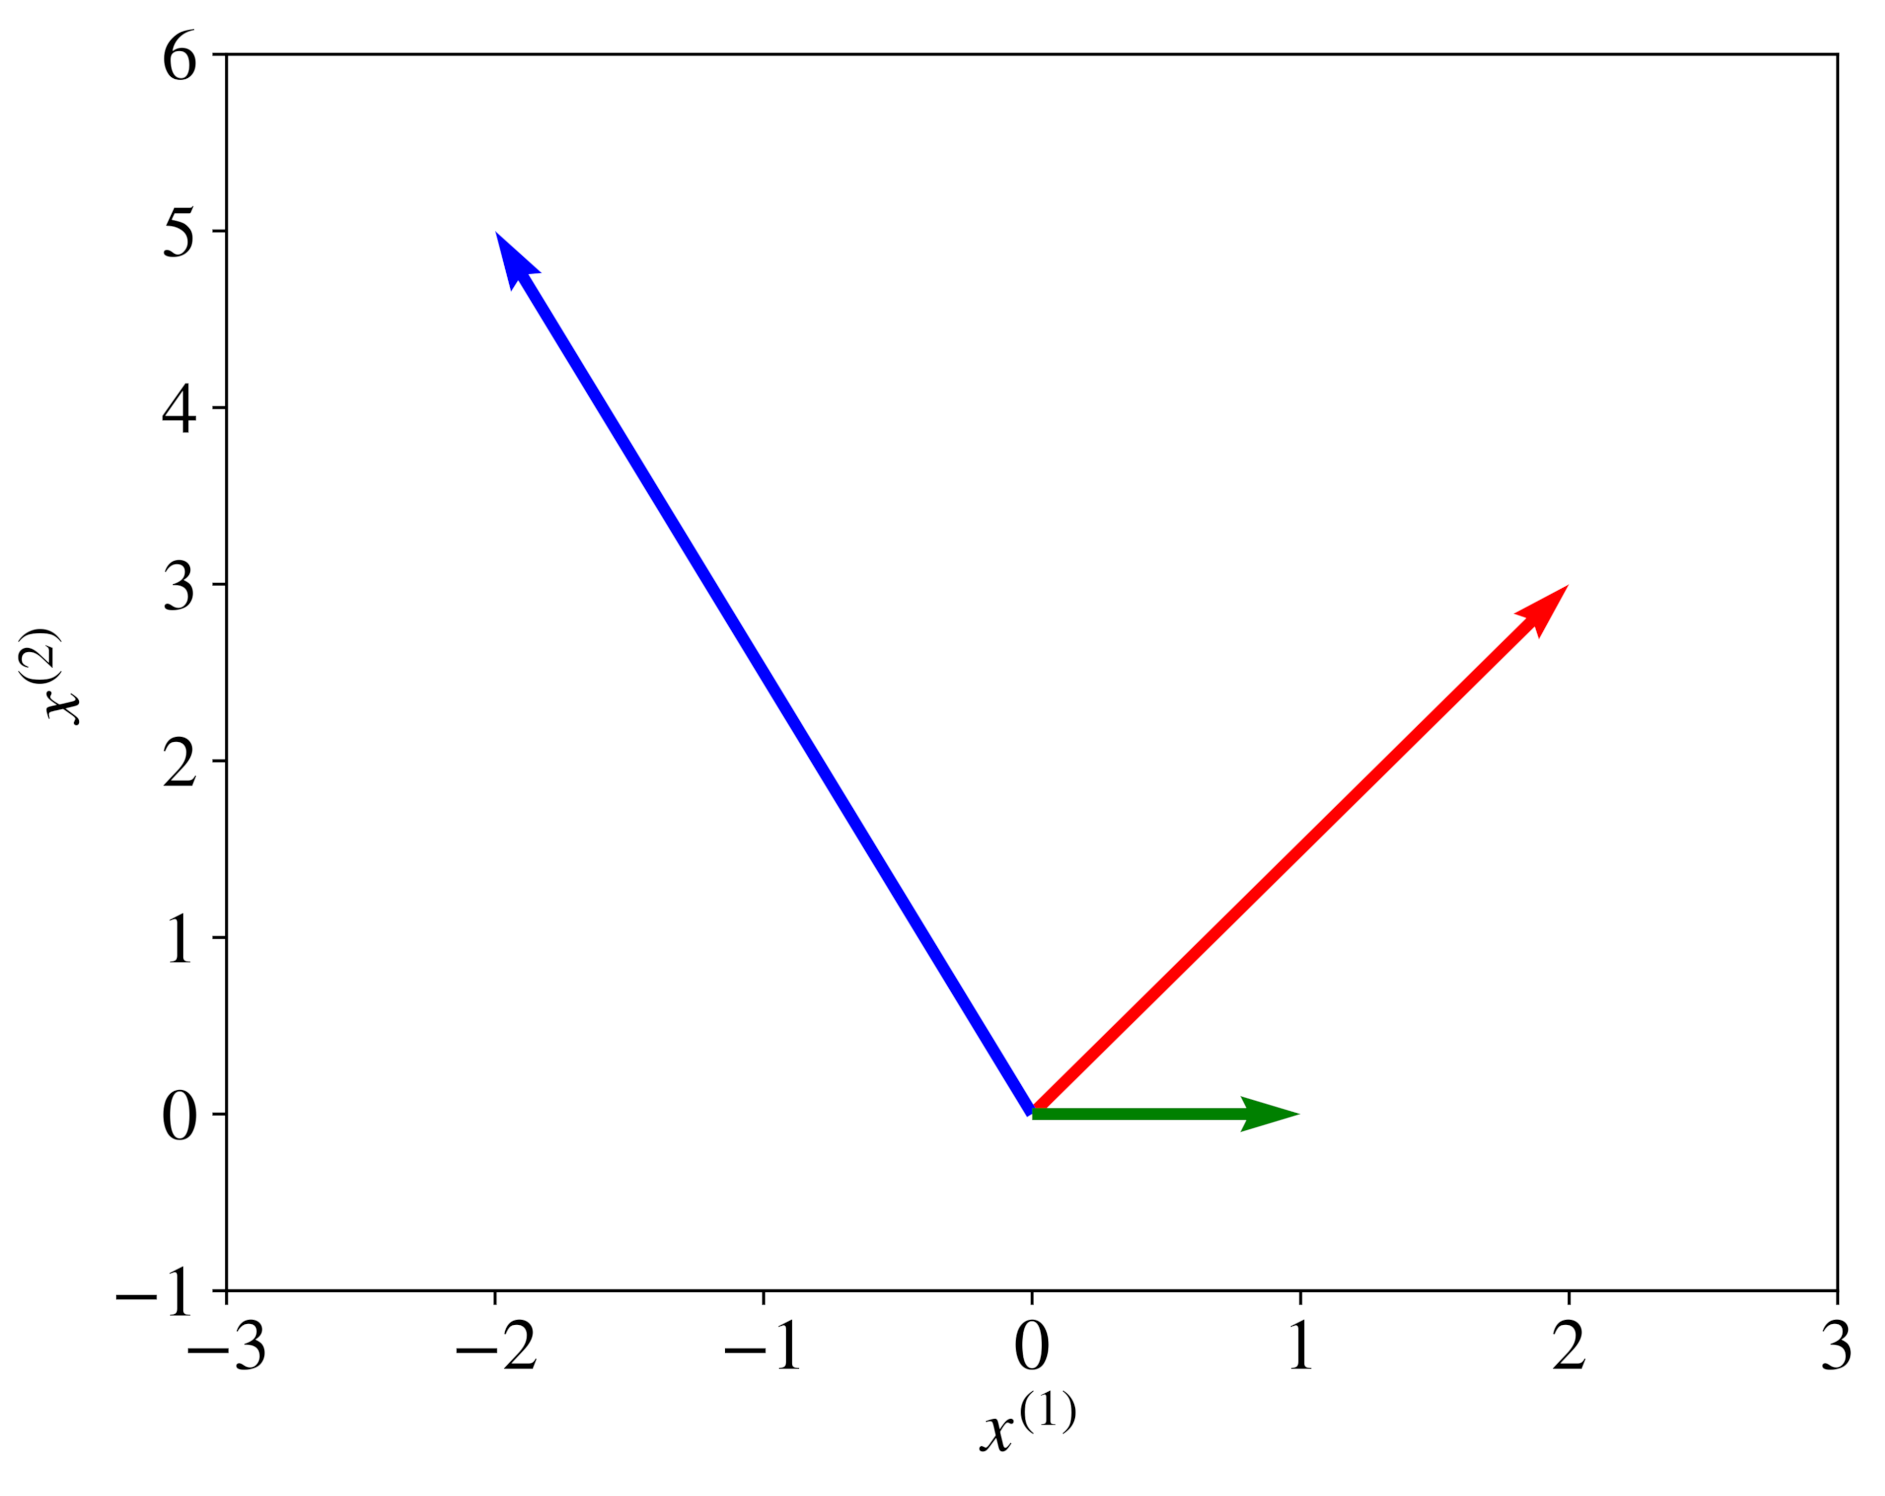
\includegraphics[width=\linewidth]{imgs/notation/notation_1}
		\caption{First subfigure}
	\end{subfigure}
	\hfill % this will put some space between your two figures
	\begin{subfigure}[t]{0.45\linewidth}
		\centering
		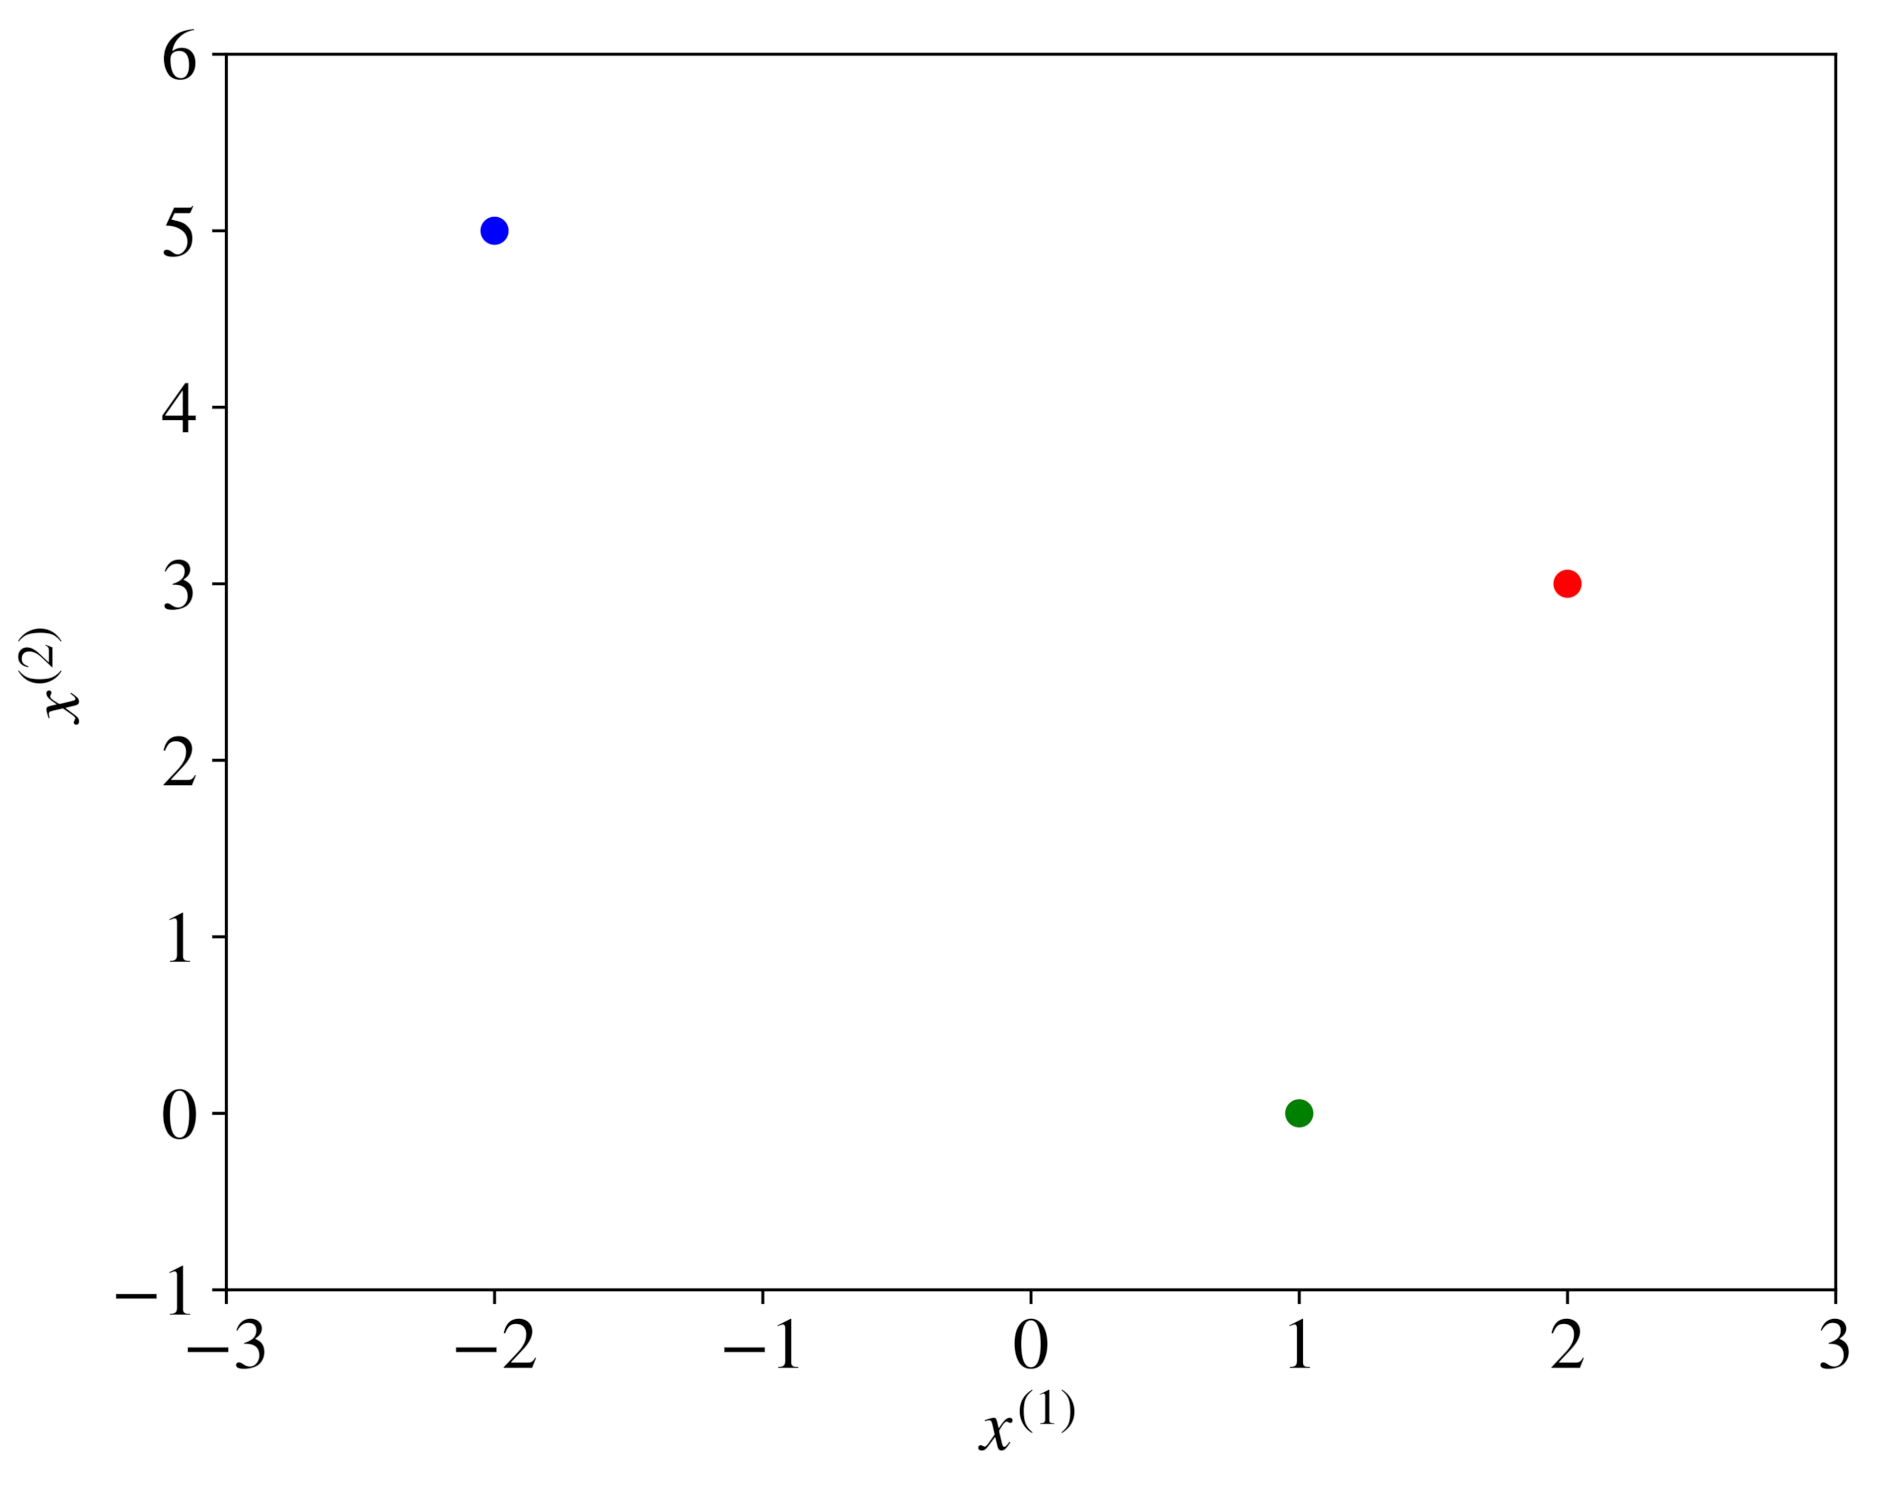
\includegraphics[width=\linewidth]{imgs/notation/notation_2}
		\caption{Second subfigure}
	\end{subfigure}
	\caption{Three vectors visualized as directions and as points.}
	\label{fig:notation_1}
\end{figure}

A \textbf{matrix} is a rectangular array of numbers arranged in rows and columns, which are denoted with bold capital letters, such as $\mathbf{A}$ or $\mathbf{W}$.  A \textbf{set} is an unordered collection of unique elements. We denote a set as a calligraphic capital character, for example, \(\mathcal{S}\). When an element belongs to a set \(\mathcal{S}\) , we write $x\in\mathcal{S}$. We can obtain a new set $\mathcal{S}_3$ as an \textbf{intersection} of two set $\mathcal{S}_1$ and $\mathcal{S}_2$, written as $\mathcal{S} \leftarrow\mathcal{S}_{1} \cap \mathcal{S}_{2}$. Also we can obtain a new set by \textbf{union}, $\mathcal{S}_3\leftarrow\mathcal{S}_1\cup\mathcal{S}_2$.

\subsection{Capital Sigma Notation}
The summation over a collection \(\mathcal{X}=\left\{x_{1}, x_{2}, \ldots, x_{n-1}, x_{n}\right\}\) or over the attributes of a vector
\(\mathbf{x}=\left[x^{(1)}, x^{(2)}, \ldots, x^{(m-1)}, x^{(m)}\right]\) is denoted like this:
\begin{equation*}
	\sum_{i=1}^{n} x_{i} \stackrel{\text { def }}{=} x_{1}+x_{2}+\ldots+x_{n-1}+x_{n}, \text { or else: } \sum_{j=1}^{m} x^{(j)} \stackrel{\text { def }}{=} x^{(1)}+x^{(2)}+\ldots+x^{(m-1)}+x^{(m)}
\end{equation*}
The notation $\stackrel{\text { def }}{=}$ means ``is defined as".

\subsection{Capital Pi Notation}